\documentclass[ % ドキュメントクラス
  platex,%upLaTeXを使う
  papersize,%紙のサイズがデフォルトと違う場合、PDFにうまく伝える
  twocolumn,
  landscape
]{jsarticle}

%% フォント関連
\usepackage[T1]{fontenc} % フォントでT1を使うこと
\usepackage{textcomp} % フォントでTS1を使うこと
\usepackage[utf8]{inputenc} % ファイルがUTF8であること
\usepackage{newpxtext,newpxmath} % ローマンと数式の字体をPalatinoに基づいた新PXフォントで
\usepackage{zi4}%等幅フォントをInconsolataで
\usepackage[multi,deluxe,jis2004]{otf}
% \usepackage[prefernoncjk]{pxcjkcat} % なるべく「半角」扱いで。
% \cjkcategory{sym18}{cjk} % sym18 (U+25A0 - U+25FF Geometric Shapes) を和文文字あつかい

%% 図表など
% 図の読みこみのために
\usepackage[dvipdfmx, hiresbb]{graphicx, xcolor}
\usepackage{booktabs} % 表の横罫線
\usepackage{lscape}  % 表などを90度回転させる

%% 囲み枠
\usepackage{tcolorbox}
\tcbuselibrary{breakable} % ページをまたいで分割できるように

% ソースコードをきれいに出力する
\usepackage{listings}
\lstset{ % 色々な設定
    language=Python, % プログラミング言語名(ここではR言語)
    basicstyle=\ttfamily, % 基本的にタイプライター体にする
    numbers=left, % 左側に行番号を表示
    numberstyle=\small, % 行番号は小さめに
    numbersep=16pt, % 行番号をどれだけ離すか
    % showspaces=true,% スペースを表示したければtrueにする
    xleftmargin=25pt, % 左側のマージン
    frame=single, %ソースコードを囲むフレーム
    framesep=10pt, %フレームとコードの間隔
    backgroundcolor=\color[gray]{0.95}, % 背景色
    breaklines=true % 長い行は改行する
}
\renewcommand{\lstlistingname}{ソースコード}

% misc
\usepackage{okumacro} % 圏点などのため
\usepackage{pxrubrica} % ルビをつける(okumacroのrubyは使わない)

% hyperrefの設定
\usepackage[dvipdfmx,%
   bookmarks=true,%PDFにしおりをつける
   bookmarksnumbered=true,%しおりに節番号などをつける
   colorlinks=false,%リンクには色をつけない
   hyperfootnotes=false,%脚注からのリンクを作らない
   pdfborder={0 0 0},%枠なし
   pdfpagemode=UseNone]{hyperref}

% PDFにしたときの文字化けを防ぐ
\usepackage{pxjahyper}

\usepackage{here}

\title{計算物理演習レポート3 サイコロゲーム}
\author{}
\date{2020年2月25日}

\begin{document}
\maketitle

\section{概要}
サイコロゲームの数値計算を行い、計算結果を理論的に考察した。

\section{チップの配布}\label{s-dist}
\subsection{計算内容}
nChip枚のチップをnPeople人に配布し、一人が持っているチップの枚数をヒストグラムでプロットする。

0~nPeople-1の番号が振られた人の誰に配布するかは、[0,1)の一様分布をnPeople倍してfloorしたものを用いた。

各パラメータは、人数nPeople = 100000, チップの枚数nChip = 10000000とした\\

\subsection{ソースコード}\label{dist-code}
以下はチップ授受のコード(\ref{s-exchange}で後述)も含む。

dice.cpp
\begin{lstlisting}[]
#include <string>
#include <iostream>
#include <iomanip>
#include "../util2.h"

using namespace std;

int main() {
    const int nPeople = 100000, nChip = 10000000;
    const long nExchange = 1000000000;
    int numsChip[nPeople] = {};

//    distribute
    for (int i = 0; i < nChip; i++) {
        int giveTo = get_random_0_to_n(nPeople);
        numsChip[giveTo] += 1;
    }
    string s1;
    for (int v : numsChip) {
        s1 += to_string(v) + "\n";
    }
    string fpath1 = "../out/dice_game/data1.dat";
    write_to_file(s1, fpath1);
//    filter(x,y)=int(x/y)*y; plot "data1.dat" u (filter($1,0.001)):(1) smooth frequency with boxes
//    でプロット

//    exchange
    cout << "Exchanging... " << flush;
    for (long i = 0; i < nExchange; i++) {
        int giveFrom, giveTo;
        do {
            giveFrom = get_random_0_to_n(nPeople);
            giveTo = get_random_0_to_n(nPeople);
        } while (giveTo == giveFrom || numsChip[giveFrom] == 0);
        numsChip[giveFrom] -= 1;
        numsChip[giveTo] += 1;
        if (i % long(double(nExchange - 1) * 0.1) == 0) {
            cout << setprecision(3) << 100.0 * double(i) / double(nExchange) << "% " << flush;
        }
    }
    string s2;
    for (int v : numsChip) {
        s2 += to_string(v) + "\n";
    }
    string fpath2 = "../out/dice_game/data2.dat";
    write_to_file(s2, fpath2);
//    binwidth=1.0; set boxwidth binwidth; bin(x,width)=width*floor(x/width); plot 'data2.dat' using (bin($1,binwidth)):(1.0) smooth freq with boxes
//    でプロット
    return 0;
}
\end{lstlisting}

util2.h
\begin{lstlisting}[]
#pragma once

#include <fstream>
#include <random>

using namespace std;

inline int get_random_0_to_n(int n) {
    // 乱数生成器
    static mt19937_64 mt64(0);

    // 0, 1, ... , n - 1 の一様分布整数生成器
    uniform_real_distribution<double> get_rand_uni_real(0.0, double(n));
    // 乱数を生成
    double numRandom = get_rand_uni_real(mt64);
    return int(floor(numRandom));
}

inline int write_to_file(const string& s, const string& fpath) {
    ofstream f;
    f.open(fpath);
    f << s;
    f.close();
    return 0;
}
\end{lstlisting}
\leavevmode\\

\subsection{計算結果}
\begin{figure}[H]
\begin{center}
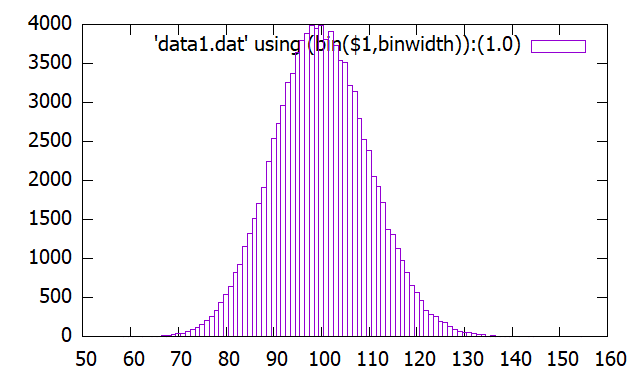
\includegraphics[width=8cm]{../cpp/out/dice_game/data1.png}
\end{center}
\caption{}
\end{figure}

\subsection{考察}
チップの枚数nChipを$M$、人数nPeopleを$N$と置く。今、一様乱数は$1,2,\cdots,N$の離散的な値に対して発生するので、一つの$x$に対して乱数の値が$x$となる確率$p$は
\begin{align}
  p=&\frac{1}{N}&
\end{align}
である。乱数を1つ作る作業を1回の試行とする。これを乱数の数$M$個分繰り返すので、$M$回試行したときには、一つの$x$に対して$k$回、乱数の値が$x$となる確率$P_M(k)$は、独立な複数回の試行より二項分布となり
\begin{align}
  P_M(k)=&{}_M \mathrm{C}_k p^k (1-p)^{M-k}&\\
\end{align}
と表せる。この二項分布のモーメントの母関数$\textrm{M}(\theta)$は
\begin{align}
  \textrm{M}(\theta)\equiv&\textrm{E}[e^{\theta k}]&\\
  =&\sum_{k=1}^{M}e^{\theta k}{}_M \mathrm{C}_k p^k (1-p)^{M-k}&\\
  =&\sum_{k=1}^{M}{}_M \mathrm{C}_k \left(pe^{\theta}\right)^k (1-p)^{M-k}&\\
  =&\left(pe^{\theta}+(1-p)\right)^M&\\
\end{align}
より、期待値$\textrm{E}[k]$は
\begin{align}
  \textrm{E}[k]\equiv&\left.\frac{\textrm{d}\textrm{M}(\theta)}{\textrm{d}\theta}\right|_{\theta\rightarrow0}&\\
  =&\left.Mpe^{\theta}\left(pe^{\theta}+(1-p)\right)^{M-1}\right|_{\theta\rightarrow0}&\\
  =&Mp&\\
  =&\frac{M}{N}&
\end{align}
分散$\sigma^{2}[k]$は$N>>1$に注意すると
\begin{align}
  \sigma^{2}[k]\equiv&\left.\frac{\textrm{d}^{2}\textrm{M}(\theta)}{\textrm{d}\theta^2}\right|_{\theta\rightarrow0}-\textrm{E}[k]^2&\\
  =&\left.\left(Mpe^{\theta}\left(pe^{\theta}+(1-p)\right)^{M-1}+M(M-1)p^{2}e^{2\theta}\left(pe^{\theta}+(1-p)\right)^{M-2}\right)\right|_{\theta\rightarrow0}&-\textrm{E}[k]^2\\
  =&Mp+M(M-1)p^{2}-(Mp)^2&\\
  =&Mp(1-p)&\\
  =&\frac{M}{N}\left(1-\frac{1}{N}\right)&\\
  =&\frac{M(N-1)}{N^2}&\\
  \sim&\frac{M}{N}&
\end{align}
より、標準偏差$\sigma[k]$は
\begin{align}
  \sigma[k]=&\sqrt{\frac{M}{N}}&
\end{align}
と表せる。$M=10000000, N=100000$を代入すると期待値$\textrm{E}[k]$と標準偏差$\sigma[k]$はそれぞれ
\begin{align}
  \textrm{E}[k]=&100&\\
  \sigma[k]=&10&
\end{align}
となる。実際に計算結果を見ると平均およそ$100$、標準偏差はおよそ$10$と読み取れるので、これは計算結果と視覚的には一致している。

実際に理論値を重ねてプロットしてみる。今、$M>>1,\textrm{E}[k]>>1,\sigma^{2}[k]>>1$より、二項分布$B(M,p)$は正規分布$N\left(Mp,Mp(1-p)\right)$で近似できるので、確率$P_M(k)$は
\begin{align}
  P_M(k)\sim&\frac{1}{\sqrt{2\pi\sigma^2}}\exp\left(-\frac{(k-Mp)^2}{2\sigma^2}\right)&\\
  =&\frac{1}{\sqrt{2\pi\frac{M}{N}}}\exp\left({-\frac{(k-\frac{M}{N})^2}{2\frac{M}{N}}}\right)&
\end{align}
と表せる。データ数Nよりヒストグラム$f(k)$は
\begin{align}
  f(k)\equiv&N\cdot P_M(k)&\\
  =&\frac{N}{\sqrt{2\pi\frac{M}{N}}}\exp\left({-\frac{(k-\frac{M}{N})^2}{2\frac{M}{N}}}\right)&\\
  =&\frac{10000}{\sqrt{2\pi}}\exp\left(-\frac{(k-100)^2}{200}\right)&\\
\end{align}
これをプロットすると
\begin{figure}[H]
\begin{center}
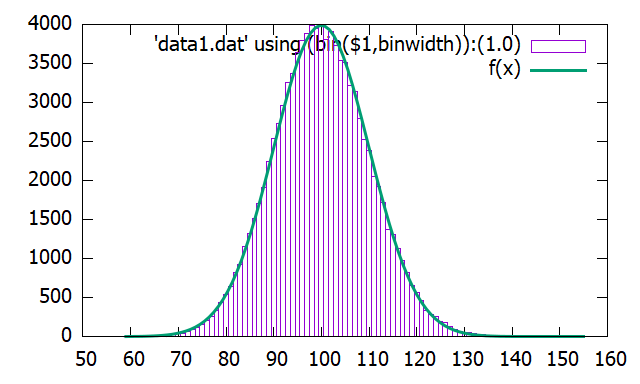
\includegraphics[width=8cm]{../cpp/out/dice_game/data1_with_theory.png}
\end{center}
\caption{計算結果(理論値付き)}
\end{figure}
となり、計算結果とよく一致している。よって計算結果は妥当といえる。

\section{チップの授受}\label{s-exchange}
\subsection{計算内容}
次に配布されたチップを交換していく。まず、\ref{s-dist}と同じの分布を使い、ランダムに2人を決定する。2人が同一人物だったり、チップをあげる人がチップを1枚も持っていなかった場合は乱数を再生成する。そしてチップを手渡す。これをnExchange回繰り返し、一人が持っているチップの枚数をヒストグラムでプロットする。

パラメータは、交換回数nExchange = 1000000000とした\\

\subsection{ソースコード}
\ref{dist-code}に既に記載。

\subsection{計算結果}
\begin{figure}[H]
\begin{center}
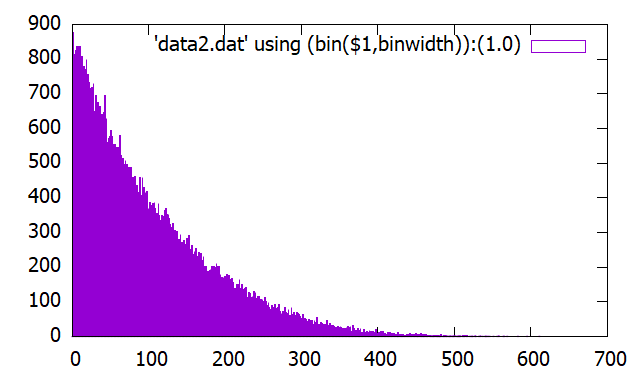
\includegraphics[width=8cm]{../cpp/out/dice_game/data2.png}
\end{center}
\caption{}
\end{figure}

\subsection{考察}
計算結果を次のようなモデルで説明する。

ミクロカノニカルアンサンブル下の量子気体の統計力学的なモデルを考える。計算でいうランダムな交換をこの系でいう粒子の衝突による振動エネルギーの変化とすると、この計算結果の分布をある一つのエネルギー準位にある粒子の数(占有数)と解釈することができる。ただし、気体は高温で密度は十分に小さく量子効果は無視できるとする。

同様にチップの枚数nChipを$M$、人数nPeopleを$N$と置く。

この系において系が平衡状態にあるとき、ある一つの粒子が離散的なエネルギー$k$である確率$p(k;N,E)$は、チップ$M$枚、人数$N$人のときにチップがどう分配されるのかを考え、「ある人の持つチップの枚数が$k$枚である確率$p(k;N,M)$」と本質的に等しいとみることができる。今回は計算可能なこれを計算していくこととする。

まず、チップの配布の総組み合わせ$W(N,M)$は、丸○がM個と仕切り|がN個の並び方と考えることができるから、
\begin{align}
  W(N,M)=\frac{(M+N-1)!}{M!(N-1)!}
\end{align}
通り。ここである人が$k$枚チップを持っている場合の
の数$W(N-1,M-k)$を考えると、残りの人の組み合わせの数を数え上げればよいから、
\begin{align}
  W(N-1,M-k)&=\frac{(M-k+N-2)!}{(M-k)!(N-2)!}&
\end{align}
通りである。よって、一つの粒子が離散的なエネルギー$k$である確率$p(k;N,M)$は、総組み合わせに対する条件付き確率であり
\begin{align}
  p(k;N,M)=&\frac{W(N-1,M-k)}{W(N,M)}&\\
  =&\frac{(M-k+N-2)!}{(M-k)!(N-2)!}\frac{M!(N-1)!}{(M+N-1)!}&\\
  \sim&\left(\frac{M-k+N-2}{e}\right)^{M-k+N-2}\left(\frac{e}{M-k}\right)^{M-k}\left(\frac{e}{N-2}\right)^{N-2}\cdot\relax&\\\nonumber&\left(\frac{M}{e}\right)^{M}\left(\frac{N-1}{e}\right)^{N-1}\left(\frac{e}{M+N-1}\right)^{M+N-1}&\\
  =&\left(\frac{M-k+N-2}{M-k}\right)^{M-k}\left(\frac{M-k+N-2}{N-2}\right)^{N-2}\left(\frac{M}{M+N-1}\right)^{M}\left(\frac{N-1}{M+N-1}\right)^{N-1}&\\
  =&\left(\frac{(M-k+N-2)M}{(M-k)(M+N-1)}\right)^{M}\left(\frac{M-k}{M-k+N-2}\right)^{k}\left(\frac{M-k+N-2}{N-2}\right)^{N-2}\left(\frac{N-1}{M+N-1}\right)^{N-1}&\\
  \sim&\left(\frac{(M+N)M}{M(M+N)}\right)^{M}\left(\frac{M}{M+N}\right)^{k}\left(\frac{M+N}{N}\right)^{N-2}\left(\frac{N}{M+N}\right)^{N-1}&\\
  =&\frac{N}{M+N}\left(\frac{M}{M+N}\right)^{k}&
\end{align}
と計算される。ただし、途中でスターリングの公式$n!\sim(\frac{n}{e})^n$、及び$M>>k$と$N>>1$を用いた。

データ数$N$より先程プロットしたヒストグラムはこの確率の関数を$N$倍したものとなる。$M=10000000, N=100000$を代入すると、
\begin{align}
  f(k)\equiv&N\cdot p(k;N,M)&\\
  =&\frac{N^2}{M+N}\left(\frac{M}{M+N}\right)^{k}&\\
  \sim&990.1\cdot0.9901^{k}&
\end{align}
これを先程の図に重ねてプロットすると
\begin{figure}[H]
\begin{center}
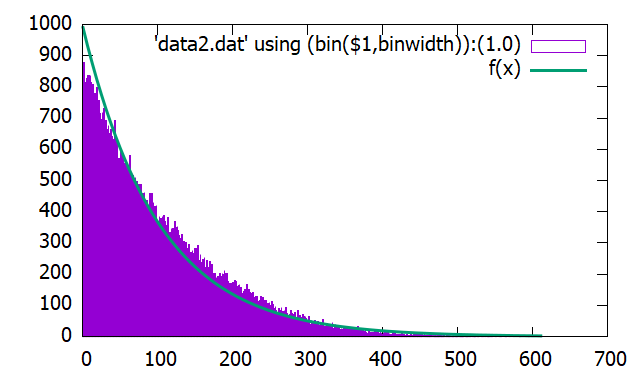
\includegraphics[width=8cm]{../cpp/out/dice_game/data2_with_theory.png}
\end{center}
\caption{計算結果(理論値付き)}
\end{figure}
となり計算結果とこのモデルで考えた理論値と概ね一致する。よって計算結果はこのモデルで考えると概ね妥当といえる。

\begin{thebibliography}{99}
\bibitem{sit}
統計力学入門の為のゲーム(課題1、2含む)
http://www.scc.kyushu-u.ac.jp/BioChemPhys/ko-gi/game09.pdf
\bibitem{random}
乱数とヒストグラム モデリングとシミュレーション
http://aoba.cc.saga-u.ac.jp/lecture/ModelingAndSimulation/PDF/Random.pdf
\bibitem{binomial}
二項分布 - Wikipedia
https://ja.wikipedia.org/wiki/二項分布
\bibitem{gaussian}
正規分布 - Wikipedia
https://ja.wikipedia.org/wiki/正規分布
\bibitem{boltzmann}
ボルツマン分布 - Wikipedia
https://ja.wikipedia.org/wiki/ボルツマン分布
\end{thebibliography}

\end{document}
